\documentclass{article}

\usepackage[ngerman]{babel}
\usepackage[T1]{fontenc}
\usepackage[utf8]{inputenc}
\usepackage{float}
\usepackage{svg}
\usepackage{amsmath}

\graphicspath{{diagrams/}}

\title{\textbf{Signale \& Systeme \\ Analyse eines IT\textsubscript{1}-Systems}}


\author{
\vspace{8em} \\
\textbf{Name:} Philipp Rall \& Duc Vo Ngoc \\
\textbf{Matrikelnr.:} XXXX   \\
\textbf{Studiengangsleiter:} Prof. Dr. Heinrich Braun\\
\textbf{Kurs:} TINF18B2 \\
\vspace{8em} 
}

\begin{document}

\maketitle
\newpage
\section{Das System}
\subsection{Die Übertragungsfunktion}

Formel \ref{eq:G(s)_1} zeigt die allgemeine Übertragungsfunktion eines $IT_1-Gliedes$.\\ In Formel \ref{eq:G(s)_2} wird ein konkretes IT1-Glied dargestellt, das in diesem Skript analysiert wird. \\ Formel \ref{eq:G(s)_3} zeigt dessen ausmultiplizierte Form.

\begin{eqnarray}
G(s) &=& \frac{Y(s)}{U(s)} \\
\label{eq:G(s)_1}
&=& \frac{K}{(T_I+T_1s)*s} \\
\label{eq:G(s)_2}
&=& \frac{4}{(1+7s)s} \\
\label{eq:G(s)_3}
&=& \frac{4}{7s^2+s}
\end{eqnarray}
\section{Eigenschaften des Systems}

Im folgenden ist eine Liste angeführt an Eigenschaften, die sich aus der Übertragungsfunktion $G(s)$ ergeben:
\begin{itemize}
	\item Differenzengrad , also Nennergrad - Zählergrad, mit Wert 2, dadurch ist das System nicht sprungfähig, antwortet aber sofort mit einer Steigung größer 0
	\item Ein $IT_1-Glied$
	\item Integrierendes Verhalten (I-Verhalten) mit einer Zeitkonstanten $T_1$
	\item Keine Nullstellen, deshalb positiver Anfang
	\item Es gibt zwei reelle Polstellen, die kleiner gleich 0 sind $\rightarrow$ das System ist stabil
\end{itemize}

\section{Darstellungsformen des Systems}
\section{Eingangs-Ausgang Differentialgleichung}

\begin{eqnarray*}
    G(s) =\frac{Y(s)}{U(s)} &=& \frac{4}{7s^2+s} \\
    Y(s)(7s^2+s) &=& U(s) * 4 \\
     7 \ddot y +  \dot y &=& 4u
\end{eqnarray*}
Anfangswerte: \(y(0)=y_0, \dot y(0)=\dot y_0, u(0)=u_0\)

\subsection{Zustandsraumdarstellung}

Die allgemeine Form der Zustandsraumdarstellung ist in den folgenden zwei Zeilen zu sehen.

\begin{eqnarray*}
	\dot x &=& Ax + Bu \\
	y &=& Cx + Du
\end{eqnarray*}

Das behandelte $IT_1-Glied$ besitzt mit den Anfangswerten \[x_1(0) = y(0),  x_2(0) = \dot y(0)\] folgende Zustandsraumdarstellung:

\begin{eqnarray*}
	\dot x &=& \left(\begin{array}{cc} 0 & 1\\ \frac{1}{7} & 0\end{array}\right) x + \left(\begin{array}{c} 0\\ -\frac{4}{7}\end{array}\right) u \\
	y &=& \left(\begin{array}{cc} 1 & 0\end{array}\right) x
\end{eqnarray*} 




UNTERSCHIEDLICH ZU MATLAB LÖSUNG???
Matlab:

\begin{eqnarray*}
	\dot x &=& \left(\begin{array}{cc} -\frac{1}{7} & 0\\ \frac{1}{4} & 0\end{array}\right) x + \left(\begin{array}{c} 2\\ 0\end{array}\right) u  \\
	y &=& \left(\begin{array}{cc} 0 & \frac{8}{7}\end{array}\right) x
\end{eqnarray*}

\section{Simulation des Systems}
\subsection{Die Übergangsfunktion}

Die Übergangsfunktion $h(t)$, auch Sprungantwort genannt, ist die Antwort im Zeitbereich auf die Heaviside-Funktion: \[\sigma (t) = \begin{cases} 0 & \text{für t < 0} \\ 1 & \text{für t > 0} \end{cases}\] \newline
In Abbildung \ref{fig:aufbau} ist der Aufbau zu sehen. Das Oszilloskop in Abbildung \ref{fig:oszilloskop} zeigt die Sprungantwort im Simulationsintervall 0 - 100 an. \newline
In Abbildung \ref{fig:matlab_sprungantwort} ist die Übergangsfunktion in Matlab vom Intervall 0 bis 3500 zu sehen, während Abbildung \ref{fig:matlab100_sprungantwort} die Sprungantwort im Intervall 0 bis 100 zeigt. \\
Die Steigung der Asymptoten der Sprungantwort entspricht dem statischen Verstärkungsfaktor $K=4$.

\begin{figure}[H]
	\centering
	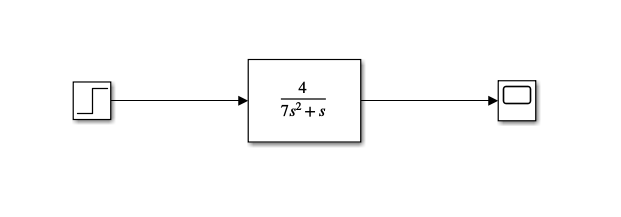
\includegraphics[width=0.8\textwidth]{{diagrams/aufbau.png}}
	\caption[Aufbau]{Aufbau in Simulink}
	\label{fig:aufbau}
\end{figure}

\begin{figure}[H]
	\centering
	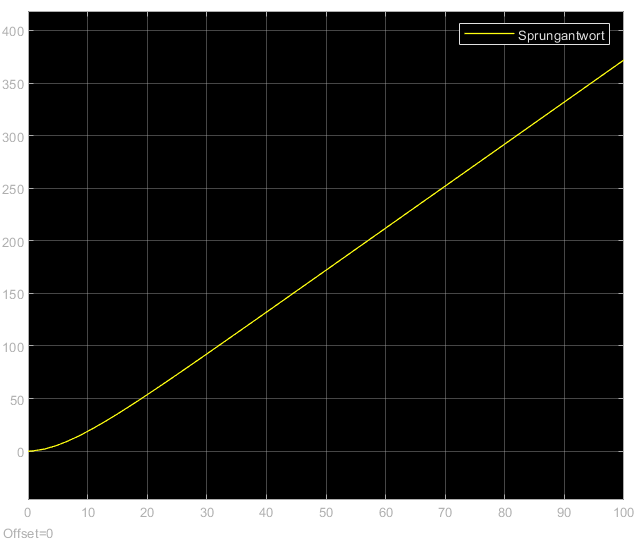
\includegraphics[width=0.8\textwidth]{{diagrams/sprungantwort_simulink_100.png}}
	\caption[Oszilloskop]{Oszilloskop - Sprungantwort im Intervall 0 bis 100}
	\label{fig:oszilloskop}
\end{figure}

\begin{figure}[H]
	\centering
	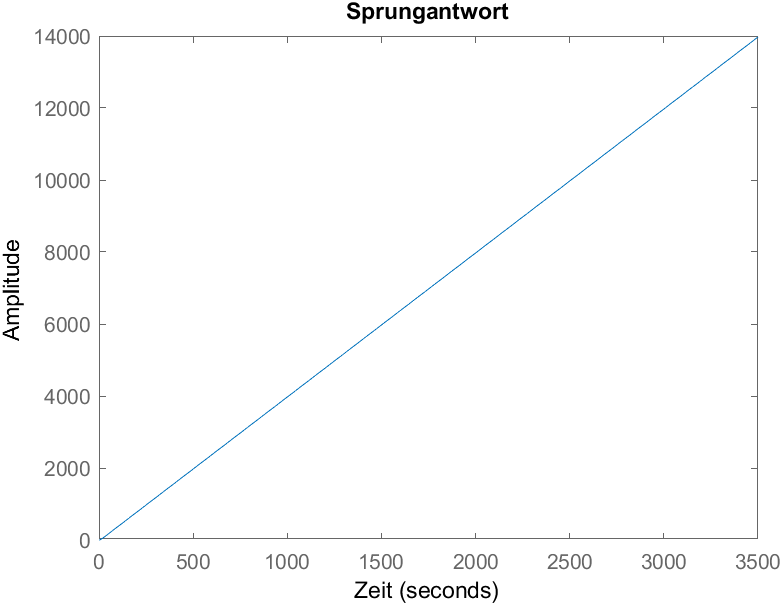
\includegraphics[width=0.8\textwidth]{{diagrams/sprungantwort_matlab.png}}
	\caption[Oszilloskop]{Matlab - Sprungantwort}
	\label{fig:matlab_sprungantwort}
\end{figure}

\begin{figure}[H]
	\centering
	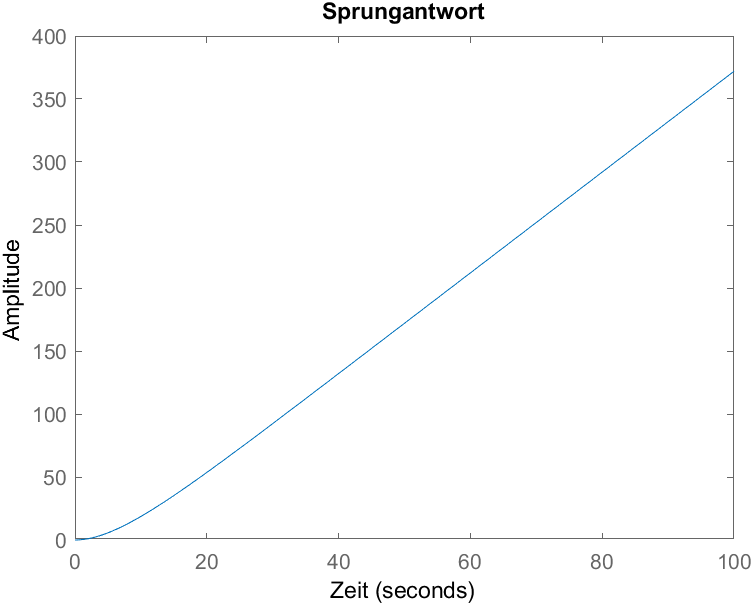
\includegraphics[width=0.8\textwidth]{{diagrams/sprungantwort_matlab_limit100.png}}
	\caption[Oszilloskop]{Matlab - Sprungantwort im Intervall 0 bis 100}
	\label{fig:matlab100_sprungantwort}
\end{figure}
\subsection{Die Gewichtsfunktion}

In Abbildung \ref{fig:impulse} ist die Gewichtsfunktion $g(t)$, auch Impulsantwort genannt, zu sehen. Diese Funktion ist die Ableitung der Übergangsfunktion $h(t)$, auch Sprungantwort genannt.
\[h(t) \xrightarrow{\frac{d}{dt}} g(t) \]
\[H(s) = \frac{1}{s} * G(s) \xrightarrow{*s} G(s)\]
Die Impulsantwort konvergiert gegen den statischen Verstärkungsfaktor $K=4$: \[lim_{t\to\infty} h(t) = K\]

\begin{figure}[H]
	\centering
	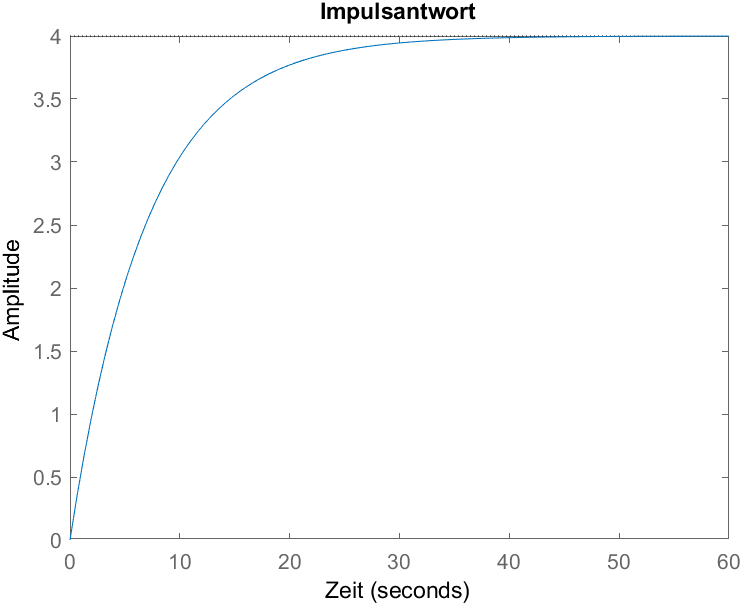
\includegraphics[width=0.8\textwidth]{{diagrams/impulseantwort.png}}
	\caption[Impulsantwort]{Impulsantwort}
	\label{fig:impulse}
\end{figure}
\subsection{Die explizite Lösung}

Durch die inverse Laplacetransformation lässt sich die explizite Lösung des Systems für die Impulsfunktion als Eingangssignal ermitteln:

\begin{eqnarray*}
	g(t) &=& L^{-1}\{\frac{4}{7s^2 + s}\} \\ 
	&=& 4 - 4*e^{-\frac{t}{7}}
\end{eqnarray*}


Durch die Integration der expliziten Lösung kommen wir auf h(t):

\begin{eqnarray*}
	h(t) &=& \int_{0}^{t}g(\tau)d\tau \\ 
	&=& 4 * t + 28*e^{-\frac{t}{7}}
\end{eqnarray*}

\subsection{Statischer Verstärkungsfaktor}

Der statischer Verstärkungsfaktor des behandelten IT1-Gliedes beträgt: \[K=4\]
Ein Graph des Verstärkungsfaktor, wobei auf der $x-Achse$ die konstanten Eingänge und auf der $y-Achse$ die Ausgänge des Systems für $t \rightarrow \infty$ aufgetragen sind, ist in Abbildung~\ref{fig:static-curve} zu sehen.

\begin{figure}[H]
	\centering
	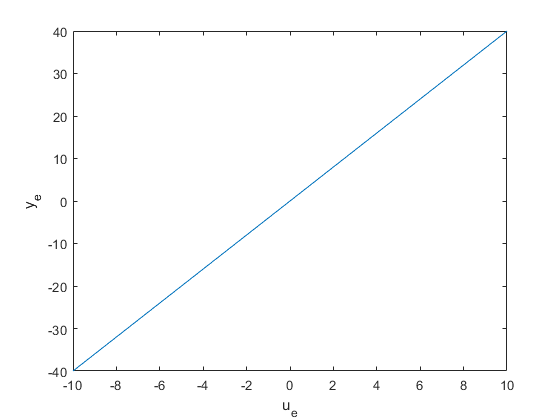
\includegraphics[width=0.7\linewidth]{{diagrams/staticCurve.png}}
	\caption[Statische Verstärkung]{Statische Verstärkung}
	\label{fig:static-curve}
\end{figure}

\section{Verhalten bei Schwingungseingängen}
\subsection{Das Pol-Nullstellenplot}

In Abbildung \ref{fig:pnp} ist das Pol-Nullstellenplot zu dem System zu sehen. Die x markierten Stellen zeigen die Polstellen an. Dieses System hat keine Nullstellen. Die Polstellen des Systems befinden sich im negativen (0 inkludiert) Teil der reell-wertigen Achse und zeigt somit, dass das System stabil ist.

\begin{figure}[H]
	\centering
	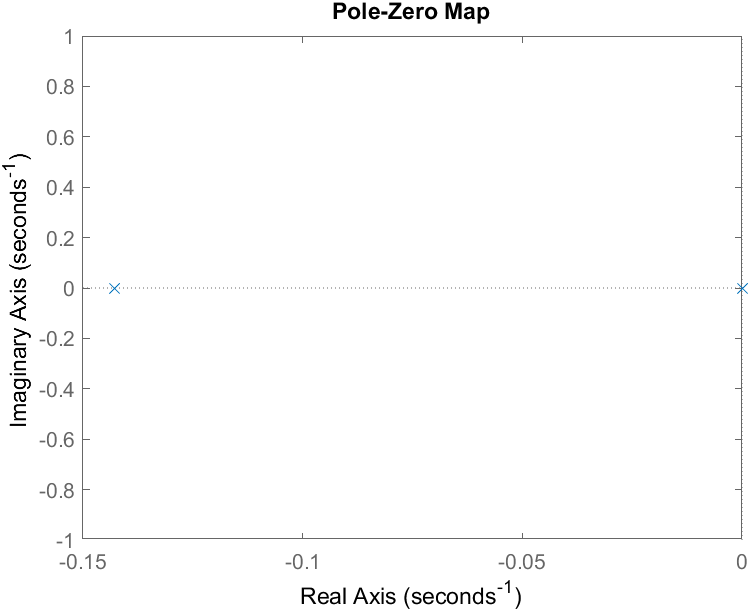
\includegraphics[width=0.8\textwidth]{{diagrams/pol_nullstellenplot.png}}
	\caption[Pol-Nullstellenplot]{Pol-Nullstellenplot}
	\label{fig:pnp}
\end{figure}
\subsection{Bode-Diagramm}

In Abbildung \ref{fig:bode-diagram} ist die Amplitude und die Phase des Systemausgangs in Abhängigkeit zur Frequenz (logarithmisch skaliert) dargestellt.

\begin{figure}[H]
	\centering
	\includegraphics[width=0.8\textwidth]{"diagrams/bode diagram"}
	\caption[Bode-Diagramm]{Bode-Diagramm}
	\label{fig:bode-diagram}
\end{figure}

\section{Nyquist-Plot}

Die Ortskurve oder auch Nyquist-Plot in Abbildung \ref{fig:nyquist-plot} ist ein Graph, der die Amplitude und Phase des Systems für Schwingungen mit allen Frequenzen darstellt.

\begin{figure}[H]
	\centering
	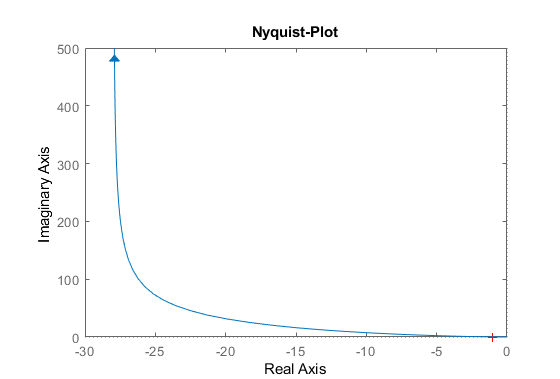
\includegraphics[width=0.7\linewidth]{diagrams/nyquistDiagram.png}
	\caption[Nyquist-Plot]{Nyquist-Plot}
	\label{fig:nyquist-plot}
\end{figure}

\end{document}